\documentclass[a4paper,14pt]{article}

%%% Работа с русским языком
\usepackage{cmap}					% поиск в PDF
\usepackage{mathtext} 				% русские буквы в формулах
\usepackage[T2A]{fontenc}			% кодировка
\usepackage[utf8]{inputenc}			% кодировка исходного текста
\usepackage[english,russian]{babel}	% локализация и переносы
\usepackage{indentfirst}
\usepackage{algorithm,algpseudocode}
\usepackage{stmaryrd}

\frenchspacing

\newcommand{\bz}{\mathbf{z}}
\newcommand{\bx}{\mathbf{x}}
\newcommand{\by}{\mathbf{y}}
\newcommand{\bv}{\mathbf{v}}
\newcommand{\bw}{\mathbf{w}}
\newcommand{\ba}{\mathbf{a}}
\newcommand{\bb}{\mathbf{b}}
\newcommand{\bp}{\mathbf{p}}
\newcommand{\bq}{\mathbf{q}}
\newcommand{\bt}{\mathbf{t}}
\newcommand{\bu}{\mathbf{u}}
\newcommand{\bT}{\mathbf{T}}
\newcommand{\bX}{\mathbf{X}}
\newcommand{\bZ}{\mathbf{Z}}
\newcommand{\bS}{\mathbf{S}}
\newcommand{\bH}{\mathbf{H}}
\newcommand{\bW}{\mathbf{W}}
\newcommand{\bY}{\mathbf{Y}}
\newcommand{\bU}{\mathbf{U}}
\newcommand{\bQ}{\mathbf{Q}}
\newcommand{\bP}{\mathbf{P}}
\newcommand{\bA}{\mathbf{A}}
\newcommand{\bB}{\mathbf{B}}
\newcommand{\bC}{\mathbf{C}}
\newcommand{\bE}{\mathbf{E}}
\newcommand{\bF}{\mathbf{F}}
\newcommand{\bomega}{\boldsymbol{\omega}}
\newcommand{\btheta}{\boldsymbol{\theta}}
\newcommand{\bgamma}{\boldsymbol{\gamma}}
\newcommand{\bdelta}{\boldsymbol{\delta}}
\newcommand{\bPsi}{\boldsymbol{\Psi}}
\newcommand{\bpsi}{\boldsymbol{\psi}}
\newcommand{\bxi}{\boldsymbol{\xi}}
\newcommand{\bchi}{\boldsymbol{\chi}}
\newcommand{\bzeta}{\boldsymbol{\zeta}}
\newcommand{\blambda}{\boldsymbol{\lambda}}
\newcommand{\beps}{\boldsymbol{\varepsilon}}
\newcommand{\bZeta}{\boldsymbol{Z}}
% mathcal
\newcommand{\cX}{\mathcal{X}}
\newcommand{\cY}{\mathcal{Y}}
\newcommand{\cW}{\mathcal{W}}

\newcommand{\dH}{\mathbb{H}}
\newcommand{\dR}{\mathbb{R}}
% transpose
\newcommand{\T}{^{\mathsf{T}}}

\renewcommand{\epsilon}{\ensuremath{\varepsilon}}
\renewcommand{\phi}{\ensuremath{\varphi}}
\renewcommand{\kappa}{\ensuremath{\varkappa}}
\renewcommand{\le}{\ensuremath{\leqslant}}
\renewcommand{\leq}{\ensuremath{\leqslant}}
\renewcommand{\ge}{\ensuremath{\geqslant}}
\renewcommand{\geq}{\ensuremath{\geqslant}}
\renewcommand{\emptyset}{\varnothing}

%%% Дополнительная работа с математикой
\usepackage{amsmath,amsfonts,amssymb,amsthm,mathtools} % AMS
\usepackage{icomma} % "Умная" запятая: $0,2$ --- число, $0, 2$ --- перечисление

%% Номера формул
%\mathtoolsset{showonlyrefs=true} % Показывать номера только у тех формул, на которые есть \eqref{} в тексте.
%\usepackage{leqno} % Нумереация формул слева

%% Свои команды
\DeclareMathOperator{\sgn}{\mathop{sgn}}

%% Перенос знаков в формулах (по Львовскому)
\newcommand*{\hm}[1]{#1\nobreak\discretionary{}
	{\hbox{$\mathsurround=0pt #1$}}{}}

%%% Работа с картинками
\usepackage{graphicx}  % Для вставки рисунков
\setlength\fboxsep{3pt} % Отступ рамки \fbox{} от рисунка
\setlength\fboxrule{1pt} % Толщина линий рамки \fbox{}
\usepackage{wrapfig} % Обтекание рисунков текстом

%%% Работа с таблицами
\usepackage{array,tabularx,tabulary,booktabs} % Дополнительная работа с таблицами
\usepackage{longtable}  % Длинные таблицы
\usepackage{multirow} % Слияние строк в таблице

%%% Теоремы
\theoremstyle{plain} % Это стиль по умолчанию, его можно не переопределять.
\newtheorem{theorem}{Теорема}[section]
\newtheorem{proposition}[theorem]{Утверждение}

\theoremstyle{definition} % "Определение"
\newtheorem{corollary}{Следствие}[theorem]
\newtheorem{problem}{Задача}[section]

\theoremstyle{remark} % "Примечание"
\newtheorem*{nonum}{Решение}

\theoremstyle{definition}
\newtheorem{definition}{Definition}[section]

\theoremstyle{remark}
\newtheorem*{properties}{Properties}

\theoremstyle{remark}
\newtheorem{example}{Example}[section]

%%% Программирование
\usepackage{etoolbox} % логические операторы

%%% Страница
\usepackage{extsizes} % Возможность сделать 14-й шрифт
\usepackage{geometry} % Простой способ задавать поля
\geometry{top=25mm}
\geometry{bottom=35mm}
\geometry{left=35mm}
\geometry{right=20mm}
%
%\usepackage{fancyhdr} % Колонтитулы
% 	\pagestyle{fancy}
%\renewcommand{\headrulewidth}{0pt}  % Толщина линейки, отчеркивающей верхний колонтитул
% 	\lfoot{Нижний левый}
% 	\rfoot{Нижний правый}
% 	\rhead{Верхний правый}
% 	\chead{Верхний в центре}
% 	\lhead{Верхний левый}
%	\cfoot{Нижний в центре} % По умолчанию здесь номер страницы

\usepackage{setspace} % Интерлиньяж
%\onehalfspacing % Интерлиньяж 1.5
%\doublespacing % Интерлиньяж 2
%\singlespacing % Интерлиньяж 1

\usepackage{lastpage} % Узнать, сколько всего страниц в документе.

\usepackage{soul} % Модификаторы начертания

\usepackage{hyperref}
\usepackage[usenames,dvipsnames,svgnames,table,rgb]{xcolor}
\hypersetup{				% Гиперссылки
	unicode=true,           % русские буквы в раздела PDF
	pdftitle={Заголовок},   % Заголовок
	pdfauthor={Автор},      % Автор
	pdfsubject={Тема},      % Тема
	pdfcreator={Создатель}, % Создатель
	pdfproducer={Производитель}, % Производитель
	pdfkeywords={keyword1} {key2} {key3}, % Ключевые слова
	colorlinks=true,       	% false: ссылки в рамках; true: цветные ссылки
	linkcolor=red,          % внутренние ссылки
	citecolor=black,        % на библиографию
	filecolor=magenta,      % на файлы
	urlcolor=cyan           % на URL
}

\usepackage{csquotes} % Еще инструменты для ссылок
\usepackage{tikz} % Работа с графикой

\usepackage[style=authoryear,maxcitenames=2,backend=biber,sorting=nty]{biblatex}
\addbibresource{references.bib}

\usepackage{multicol} % Несколько колонок

\usepackage{pgfplots}
\usepackage{pgfplotstable}


\author{Vladimirov Eduard, group М05-304а}
\title{\textbf{Tensor models, tensor decomposition, and approximation}}
\date{\today}

\begin{document}
	\maketitle
	
	\begin{abstract}
		This essay explores fundamental tensor models, specifically focusing on CP and Tucker Decomposition, alongside Tensor Canonical Correlation Analysis (Tensor CCA). We introduce essential notation and operations, review core tensor decompositions, and provide insights into applications and theoretical underpinnings of tensor approximations in data science.
	\end{abstract}
	
	\section{Introduction}
	Tensors, as multidimensional generalizations of matrices, are foundational in modern data science applications such as chemometrics, neuroscience, and machine learning. Tensor decompositions, including CP and Tucker Decomposition, extend concepts of linear algebra, such as the Singular Value Decomposition (SVD), to higher-dimensional arrays. Tensor CCA, a recent advancement, generalizes canonical correlation analysis to handle data from multiple views or sources.
	
	\section{Notation and Basic Operations}
	Following the conventions of multilinear algebra, tensors are denoted by boldface Euler script letters (e.g., $\mathcal{X}$), matrices by bold uppercase letters (e.g., $\mathbf{A}$), and vectors by bold lowercase letters (e.g., $\mathbf{a}$). A scalar entry within a tensor $\mathcal{X}$ is represented as $x_{i_1 i_2 \dots i_N}$.
	
	\subsection{Mode-\( n \) Product}
	
	Let \(\mathcal{X} \in \mathbb{R}^{I_1 \times I_2 \times \dots \times I_N}\) be an \( N \)-dimensional tensor. The \textit{mode-\( n \) product} of \(\mathcal{X}\) with a matrix \(\mathbf{U} \in \mathbb{R}^{J \times I_n}\) is denoted by \( \mathcal{X} \times_n \mathbf{U} \) and results in a new tensor of size \(I_1 \times \dots \times I_{n-1} \times J \times I_{n+1} \times \dots \times I_N\). Formally, it is defined as:
	
	
	\[
	(\mathcal{X} \times_n \mathbf{U})_{i_1 \dots i_{n-1} j i_{n+1} \dots i_N} = \sum_{i_n=1}^{I_n} x_{i_1 i_2 \dots i_N} u_{j i_n}.
	\]
	
	This operation transforms the \( n \)-th mode of \(\mathcal{X}\) by multiplying it with the matrix \(\mathbf{U}\), while leaving other modes unchanged.
	
	\subsection{Kronecker Product}
	
	The \textit{Kronecker product} of two matrices \(\mathbf{A} \in \mathbb{R}^{I \times J}\) and \(\mathbf{B} \in \mathbb{R}^{K \times L}\), denoted by \(\mathbf{A} \otimes \mathbf{B}\), is a block matrix of size \((I \cdot K) \times (J \cdot L)\). Formally, the Kronecker product is defined as:
	
	\[
	\mathbf{A} \otimes \mathbf{B} = 
	\begin{bmatrix}
		a_{11} \mathbf{B} & a_{12} \mathbf{B} & \cdots & a_{1J} \mathbf{B} \\
		a_{21} \mathbf{B} & a_{22} \mathbf{B} & \cdots & a_{2J} \mathbf{B} \\
		\vdots & \vdots & \ddots & \vdots \\
		a_{I1} \mathbf{B} & a_{I2} \mathbf{B} & \cdots & a_{IJ} \mathbf{B} \\
	\end{bmatrix}.
	\]
	
	The Kronecker product is widely used in tensor computations and is essential for expressing certain operations in tensor decompositions.
	
	\subsection{Khatri-Rao Product}
	
	The \textit{Khatri-Rao product} of two matrices \(\mathbf{A} \in \mathbb{R}^{I \times K}\) and \(\mathbf{B} \in \mathbb{R}^{J \times K}\), denoted by \(\mathbf{A} \odot \mathbf{B}\), is the column-wise Kronecker product, producing a matrix of size \((I \cdot J) \times K\). Formally, the Khatri-Rao product is defined as:
	
	\[
	\mathbf{A} \odot \mathbf{B} = 
	\begin{bmatrix}
		\mathbf{a}_1 \otimes \mathbf{b}_1 & \mathbf{a}_2 \otimes \mathbf{b}_2 & \cdots & \mathbf{a}_K \otimes \mathbf{b}_K
	\end{bmatrix},
	\]
	
	where \(\mathbf{a}_k\) and \(\mathbf{b}_k\) are the \(k\)-th columns of \(\mathbf{A}\) and \(\mathbf{B}\), respectively. The Khatri-Rao product is often used in CP decomposition and tensor computations due to its role in forming compact expressions for multi-mode tensor products.
	
	\subsection{Mode-\( n \) Matricization (Unfolding)}
	
	To apply matrix operations to a tensor, we often need to convert the tensor into a matrix format, a process known as \textit{matricization} or \textit{unfolding}. The mode-\( n \) matricization of a tensor \(\mathcal{X}\), denoted as \(\mathbf{X}_{(n)}\), rearranges \(\mathcal{X}\) into a matrix by aligning the \( n \)-th mode as rows and the other modes as columns. Specifically, for a tensor \(\mathcal{X} \in \mathbb{R}^{I_1 \times I_2 \times \dots \times I_N}\), the mode-\( n \) matricization \(\mathbf{X}_{(n)}\) is a matrix of size \(I_n \times \left( \prod_{k \neq n} I_k \right)\), defined as:
	
	\[
	\mathbf{X}_{(n)}(i_n, j) = x_{i_1 i_2 \dots i_N}
	\]
	
	where \( j = 1 + \sum_{k=1, k \neq n}^N (i_k - 1) J_k \) and \( J_k = \prod_{m=1}^{k-1} I_m \) for \( k < n \).
	
	\subsection{Example: Mode-3 Matricization of a 3rd-Order Tensor}
	
	For a third-order tensor \(\mathcal{X} \in \mathbb{R}^{I \times J \times K}\), the mode-3 matricization \(\mathbf{X}_{(3)}\) would rearrange \(\mathcal{X}\) into a matrix of size \(K \times (I \cdot J)\), such that:
	
	\[
	\mathbf{X}_{(1)}(i, j + (k-1)J) = x_{ijk}.
	\]
	
	\[
	\mathbf{X}_{(2)}(j, i + (k-1)I) = x_{ijk}.
	\]
	
	\[
	\mathbf{X}_{(3)}(k, i + (j-1)I) = x_{ijk}.
	\]
	
	The concept is easier to understand using an example. Let the frontal slices of \( \mathcal{X} \in \mathbb{R}^{3 \times 4 \times 2} \) be
	
	\begin{equation}
		\mathcal{X}_1 = 
		\begin{bmatrix}
			1 & 4 & 7 & 10 \\
			2 & 5 & 8 & 11 \\
			3 & 6 & 9 & 12 
		\end{bmatrix}
		, \quad
		\mathcal{X}_2 = 
		\begin{bmatrix}
			13 & 16 & 19 & 22 \\
			14 & 17 & 20 & 23 \\
			15 & 18 & 21 & 24 
		\end{bmatrix}.
	\end{equation}
	
	Then the three mode-\( n \) unfoldings are
	
	\[
	\mathcal{X}_{(1)} = 
	\begin{bmatrix}
		1 & 4 & 7 & 10 & 13 & 16 & 19 & 22 \\
		2 & 5 & 8 & 11 & 14 & 17 & 20 & 23 \\
		3 & 6 & 9 & 12 & 15 & 18 & 21 & 24 
	\end{bmatrix}
	,
	\]
	
	\[
	\mathcal{X}_{(2)} = 
	\begin{bmatrix}
		1 & 2 & 3 & 13 & 14 & 15 \\
		4 & 5 & 6 & 16 & 17 & 18 \\
		7 & 8 & 9 & 19 & 20 & 21 \\
		10 & 11 & 12 & 22 & 23 & 24 
	\end{bmatrix}
	,
	\]
	
	\[
	\mathcal{X}_{(3)} = 
	\begin{bmatrix}
		1 & 2 & 3 & \dots & 9 & 10 & 11 & 12 \\
		13 & 14 & 15 & \dots & 21 & 22 & 23 & 24 
	\end{bmatrix}.
	\]
	
	\subsection{Properties of Mode-\( n \) Product and Matricization}
	
	1. \textit{Associativity:} The mode-\( n \) product is associative with respect to matrix multiplication:
	\[
	(\mathcal{X} \times_n \mathbf{U}) \times_n \mathbf{V} = \mathcal{X} \times_n (\mathbf{V} \mathbf{U}).
	\]
	
	2. \textit{Commutativity:} For distinct modes
	in a series of multiplications, the order of the multiplication is irrelevant:
	
	\[
	\mathcal{X} \times_m \mathbf{A} \times_n \mathbf{B} = \mathcal{X} \times_n \mathbf{B} \times_m \mathbf{A} \quad (m \neq n).
	\]
	
	3. \textit{Relation to Matricization:} The mode-\( n \) product can be expressed using mode-\( n \) matricization. Specifically, the mode-\( n \) product of \(\mathcal{X}\) with \(\mathbf{U}\) can be represented as:
	\[
	(\mathcal{X} \times_n \mathbf{U})_{(n)} = \mathbf{U} \, \mathbf{X}_{(n)}.
	\]
	
	4. \textit{Inverse Operation:} If \(\mathbf{U}\) is invertible, the mode-\( n \) product can be reversed by multiplying with \(\mathbf{U}^{-1}\):
	\[
	\mathcal{X} = (\mathcal{X} \times_n \mathbf{U}) \times_n \mathbf{U}^{-1}.
	\]
	
	These operations are essential in tensor decompositions like CP and Tucker, where tensors are factorized through mode-\( n \) products and mode-\( n \) matricization enables matrix-based transformations.
	
	\section{CP Decomposition}
	
	\begin{figure}
		\centering
		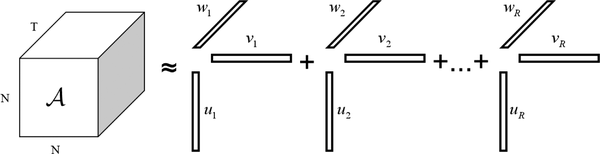
\includegraphics[width=\textwidth]{illustration-of-cp-decomposition}
		\caption{CP Decomposition}
	\end{figure}
	
	The CANDECOMP/PARAFAC (Canonical decomposition + Parallel factor analysis or CP) decomposition, is one of the fundamental tensor decomposition methods, widely used in multilinear algebra, data analysis, and machine learning. It generalizes the concept of matrix rank decomposition to tensors by expressing a tensor as a sum of rank-one components. Given a tensor \(\mathcal{X} \in \mathbb{R}^{I_1 \times I_2 \times \dots \times I_N}\), the CP decomposition seeks to approximate \(\mathcal{X}\) as follows:
	
	\begin{equation}
		\mathcal{X} \approx \sum_{r=1}^R \lambda_r \mathbf{a}^{(1)}_r \circ \mathbf{a}^{(2)}_r \circ \dots \circ \mathbf{a}^{(N)}_r,
	\end{equation}
	
	where:
	\begin{itemize}
		\item \( R \) is the rank of the decomposition, representing the smallest number of rank-one tensors that approximate \(\mathcal{X}\) with acceptable accuracy.
		\item \(\lambda_r\) are scalar weights for each rank-one component.
		\item \(\mathbf{a}^{(n)}_r \in \mathbb{R}^{I_n}\) are vectors associated with the \( n \)-th mode for each rank-\( r \) component.
		\item \( \circ \) denotes the outer product operation.
	\end{itemize}
	
	Thus, each term \(\lambda_r \mathbf{a}^{(1)}_r \circ \mathbf{a}^{(2)}_r \circ \dots \circ \mathbf{a}^{(N)}_r\) is a rank-one tensor, and their sum provides an approximation of \(\mathcal{X}\).
	
	\subsection{Rank of a Tensor and Uniqueness}
	
	The \textit{rank} of a tensor \(\mathcal{X}\), denoted as \(\text{rank}(\mathcal{X})\), is defined as the minimum number of rank-one tensors required to represent \(\mathcal{X}\) exactly (or approximately in the case of noise or incomplete data). Unlike matrices, tensors of higher order (order \( N \geq 3 \)) do not have a unique rank in general, but under certain conditions, CP decomposition is unique up to scaling and permutation of components. This uniqueness is advantageous for applications where interpretability of components is essential.
	
	\subsection{Notation and Matrix Representation}
	
	To facilitate computations, the CP decomposition can also be represented in matrix form using mode-\( n \) unfoldings of \(\mathcal{X}\). Let \(\mathbf{X}_{(n)}\) denote the mode-\( n \) matricization of \(\mathcal{X}\). Then, the CP decomposition can be represented as:
	
	\begin{equation}
		\mathbf{X}_{(n)} \approx \mathbf{A}^{(n)} \mathbf{\Lambda} \left( \mathbf{A}^{(N)} \odot \dots \odot \mathbf{A}^{(n+1)} \odot \mathbf{A}^{(n-1)} \odot \dots \odot \mathbf{A}^{(1)} \right)^T,
	\end{equation}
	
	where:
	\begin{itemize}
		\item \(\mathbf{A}^{(n)} = [\mathbf{a}^{(n)}_1, \mathbf{a}^{(n)}_2, \dots, \mathbf{a}^{(n)}_R] \in \mathbb{R}^{I_n \times R}\) is the factor matrix for the \(n\)-th mode.
		\item \(\mathbf{\Lambda} = \text{diag}(\lambda_1, \lambda_2, \dots, \lambda_R)\) is a diagonal matrix containing the weights \(\lambda_r\).
		\item \(\odot\) denotes the Khatri-Rao product, which is the column-wise Kronecker product of matrices.
	\end{itemize}
	
	This matrix form is commonly used in numerical methods to compute the CP decomposition efficiently.
	
	\subsection{Algorithms for Computing CP Decomposition}
	
	Several algorithms exist for computing the CP decomposition. The most popular methods include:
	
	\subsubsection{Alternating Least Squares (ALS)}
	
	The Alternating Least Squares (ALS) algorithm iteratively updates each factor matrix \(\mathbf{A}^{(n)}\) while keeping other factors fixed. The objective is to minimize the difference between \(\mathcal{X}\) and its approximation. The ALS update for each factor \(\mathbf{A}^{(n)}\) is computed by solving a least-squares problem for \(\mathbf{X}_{(n)}\) with respect to \(\mathbf{A}^{(n)}\).
	
	The ALS algorithm repeats this process for each mode until convergence, with the cost function given by:
	
	\[
	\min_{\mathbf{A}^{(1)}, \mathbf{A}^{(2)}, \dots, \mathbf{A}^{(N)}} \left\| \mathcal{X} - \sum_{r=1}^R \lambda_r \mathbf{a}^{(1)}_r \circ \mathbf{a}^{(2)}_r \circ \dots \circ \mathbf{a}^{(N)}_r \right\|^2.
	\]
	
	\begin{algorithm}
		\caption{CP-ALS Algorithm}
		\label{alg:CP_ALS}
		\begin{algorithmic}
			\Procedure{CP-ALS}{$\mathcal{X}, R$}
			\State Initialize $\mathbf{A}^{(n)} \in \mathbb{R}^{I_n \times R}$ for $n = 1, \dots, N$
			\Repeat
			\For{$n = 1, \dots, N$}
			\State $\mathbf{V} \leftarrow \mathbf{A}^{(1)^T} \mathbf{A}^{(1)} \ast \dots \ast \mathbf{A}^{(n-1)^T} \mathbf{A}^{(n-1)} \ast \mathbf{A}^{(n+1)^T} \mathbf{A}^{(n+1)} \ast \dots \ast \mathbf{A}^{(N)^T} \mathbf{A}^{(N)}$
			\State $\mathbf{A}^{(n)} \leftarrow \mathcal{X}_{(n)} (\mathbf{A}^{(N)} \odot \dots \odot \mathbf{A}^{(n+1)} \odot \mathbf{A}^{(n-1)} \odot \dots \odot \mathbf{A}^{(1)}) \mathbf{V}^{\dagger}$
			\State Normalize columns of $\mathbf{A}^{(n)}$ (storing norms as $\lambda$)
			\EndFor
			\Until{fit ceases to improve or maximum iterations exhausted}
			\State \Return $\lambda, \mathbf{A}^{(1)}, \mathbf{A}^{(2)}, \dots, \mathbf{A}^{(N)}$
			\EndProcedure
		\end{algorithmic}
	\end{algorithm}
	
	\subsubsection{Gradient-Based Optimization}
	
	In cases where ALS fails to converge or is inefficient, gradient-based optimization methods, such as stochastic gradient descent (SGD) or Adam, can be used to minimize the reconstruction error. These methods apply gradients directly to each factor matrix \(\mathbf{A}^{(n)}\) and the weight vector \(\boldsymbol{\lambda}\) to optimize the objective function.
	
	\subsubsection{Other Methods}
	
	Other methods include Tensor Power Iteration and methods based on higher-order orthogonal iteration (HOOI), though these are more common for Tucker decomposition.
	
	\subsection{Challenges in CP Decomposition}
	
	CP decomposition, while widely used, has challenges. Finding the correct rank \( R \) is difficult and often requires heuristics or cross-validation. Additionally, ALS can converge slowly or get stuck in local minima, and the decomposition may be sensitive to noise or missing values. Nevertheless, CP decomposition remains a powerful tool for analyzing multi-dimensional data in a structured and interpretable way.
	
	\section{Tucker Decomposition}
	
	\begin{figure}
		\centering
		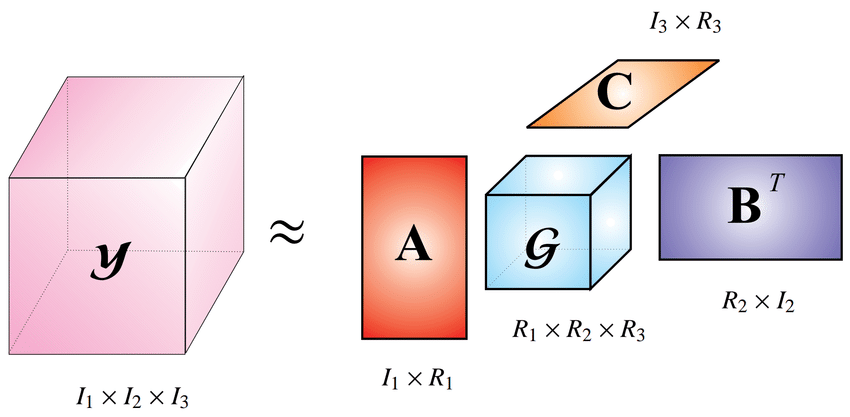
\includegraphics[width=\textwidth]{illustration-of-tucker-decomposition}
		\caption{Tucker Decomposition}
	\end{figure}

	The Tucker decomposition is a powerful tool in tensor decomposition that generalizes both Principal Component Analysis (PCA) and higher-order tensor decomposition methods. Also known as the \textit{higher-order singular value decomposition} (HOSVD) or \textit{multilinear SVD}, Tucker decomposition represents a tensor as a core tensor multiplied by factor matrices along each mode. This decomposition is particularly useful for dimensionality reduction and extracting latent factors in multi-way data.
	
	\subsection{Definition of Tucker Decomposition}
	
	Given an \( N \)-dimensional tensor \( \mathcal{X} \in \mathbb{R}^{I_1 \times I_2 \times \dots \times I_N} \), the Tucker decomposition approximates \( \mathcal{X} \) as:
	
	\begin{equation}
		\mathcal{X} \approx \mathcal{G} \times_1 \mathbf{A}^{(1)} \times_2 \mathbf{A}^{(2)} \times_3 \dots \times_N \mathbf{A}^{(N)} = \llbracket \mathcal{G}; \mathbf{A}^{(1)}, \mathbf{A}^{(2)}, \ldots, \mathbf{A}^{(N)} \rrbracket,
		\label{eq:tucker_decomposition}
	\end{equation}
	
	where:
	\begin{itemize}
		\item \( \mathcal{G} \in \mathbb{R}^{R_1 \times R_2 \times \dots \times R_N} \) is the \textit{core tensor}, which captures the interactions between the components in each mode.
		\item \( \mathbf{A}^{(n)} \in \mathbb{R}^{I_n \times R_n} \) are the factor matrices, also called projection or loading matrices, which map the original space to a reduced space for each mode \( n = 1, \dots, N \).
		\item \( \times_n \) denotes the mode-\( n \) product.
	\end{itemize}
	
	In Tucker decomposition, the dimensions \( R_n \) of the core tensor \( \mathcal{G} \) are usually smaller than the corresponding dimensions \( I_n \) of \( \mathcal{X} \), making the decomposition an efficient and compressed representation of \( \mathcal{X} \).
	
	The matrisized version of (\ref{eq:tucker_decomposition}) is
	
	\[
	\mathbf{X}_{(n)} \approx \mathbf{A}^{(n)} \mathcal{G}_{(n)} \left( \mathbf{A}^{(N)} \otimes \dots \otimes \mathbf{A}^{(n+1)} \otimes \mathbf{A}^{(n-1)} \otimes \dots \otimes \mathbf{A}^{(1)} \right)^T,
	\]
	
	This matricized form is useful in computations as it simplifies the operations on the tensor to matrix multiplications, making it easier to implement and understand.
	
	\subsection{Interpretation of Tucker Decomposition}
	
	The Tucker decomposition can be interpreted as a form of dimensionality reduction in which each mode of the tensor is reduced by projecting it onto a lower-dimensional subspace. The core tensor \( \mathcal{G} \) represents the compressed version of the original tensor, while the factor matrices \( \mathbf{A}^{(n)} \) provide the basis for reconstructing the original data from the core tensor.
	
	The core tensor can be thought of as capturing the "interactions" among the latent factors identified in each mode, while each factor matrix contains the principal components for its corresponding mode. Therefore, Tucker decomposition generalizes the concept of PCA to higher-order data structures.
	
	\subsection{Algorithms for Computing Tucker Decomposition}
	
	Various algorithms exist for computing the Tucker decomposition, with two prominent methods being:
	
	\subsection{HOSVD Algorithm}
	
	The Higher-Order Singular Value Decomposition (HOSVD) is a direct algorithm for Tucker decomposition. HOSVD performs SVD on each mode's matricization independently, providing an orthogonal basis for each mode. Here’s the step-by-step procedure for HOSVD:
	
	\begin{algorithm}
		\caption{HOSVD}
		\label{alg:HOSVD}
		\begin{algorithmic}
			\Procedure{HOSVD}{$\mathcal{X}, R_1, R_2, \dots, R_N$}
			\For{$n = 1, \dots, N$}
			\State $\mathbf{A}^{(n)} \leftarrow R_n$ leading left singular vectors of $\mathcal{X}_{(n)}$
			\EndFor
			\State $\mathcal{G} \leftarrow \mathcal{X} \times_1 \mathbf{A}^{(1)^T} \times_2 \mathbf{A}^{(2)^T} \dots \times_N \mathbf{A}^{(N)^T}$
			\State \Return $\mathcal{G}, \mathbf{A}^{(1)}, \mathbf{A}^{(2)}, \dots, \mathbf{A}^{(N)}$
			\EndProcedure
		\end{algorithmic}
	\end{algorithm}
	
	In the HOSVD algorithm, the tensor \(\mathcal{X}\) is first matricized along each mode to form \(\mathcal{X}_{(n)}\). Then, SVD is applied to each matricization independently, selecting the leading \(R_n\) singular vectors for each mode. This yields the factor matrices \(\mathbf{A}^{(1)}, \mathbf{A}^{(2)}, \dots, \mathbf{A}^{(N)}\), which are then used to compute the core tensor \(\mathcal{G}\) through mode-\(n\) products.
	
	\subsection{HOOI Algorithm}
	
	The Higher-Order Orthogonal Iteration (HOOI) is an iterative refinement method that starts with an initial guess from HOSVD and iteratively improves the factor matrices to minimize reconstruction error. HOOI typically yields a more accurate approximation of the tensor at a higher computational cost.
	
	\begin{algorithm}
		\caption{HOOI}
		\label{alg:HOOI}
		\begin{algorithmic}
			\Procedure{HOOI}{$\mathcal{X}, R_1, R_2, \dots, R_N$}
			\State Initialize $\mathbf{A}^{(n)} \in \mathbb{R}^{I_n \times R_n}$ for $n = 1, \dots, N$ using HOSVD
			\Repeat
			\For{$n = 1, \dots, N$}
			\State $\mathcal{Y} \leftarrow \mathcal{X} \times_1 \mathbf{A}^{(1)^T} \times \dots \times_{n-1} \mathbf{A}^{(n-1)^T} \times_{n+1} \mathbf{A}^{(n+1)^T} \dots \times_N \mathbf{A}^{(N)^T}$
			\State $\mathbf{A}^{(n)} \leftarrow R_n$ leading left singular vectors of $\mathcal{Y}_{(n)}$
			\EndFor
			\Until{fit ceases to improve or maximum iterations exhausted}
			\State $\mathcal{G} \leftarrow \mathcal{X} \times_1 \mathbf{A}^{(1)^T} \times_2 \mathbf{A}^{(2)^T} \dots \times_N \mathbf{A}^{(N)^T}$
			\State \Return $\mathcal{G}, \mathbf{A}^{(1)}, \mathbf{A}^{(2)}, \dots, \mathbf{A}^{(N)}$
			\EndProcedure
		\end{algorithmic}
	\end{algorithm}
	
	The initial factor matrices \(\mathbf{A}^{(n)}\) are obtained using HOSVD. Each iteration then refines \(\mathbf{A}^{(n)}\) by updating it to the \(R_n\) leading singular vectors of the mode-\(n\) unfolding \(\mathcal{Y}_{(n)}\) of the partially reconstructed tensor \(\mathcal{Y}\).
	
	The algorithm is called "Orthogonal" because it solves the following optimization problem:
	
	\[
	\begin{aligned}
		\min_{\mathcal{G}, \mathbf{A}^{(1)}, \ldots, \mathbf{A}^{(N)}} 
		&\left\| \mathcal{X} - \llbracket \mathcal{G}; \mathbf{A}^{(1)}, \mathbf{A}^{(2)}, \ldots, \mathbf{A}^{(N)} \rrbracket \right\| \\
		\text{subject to} \quad 
		&\mathcal{G} \in \mathbb{R}^{R_1 \times R_2 \times \cdots \times R_N}, \\
		&\mathbf{A}^{(n)} \in \mathbb{R}^{I_n \times R_n} \quad \text{and columnwise orthogonal for } n = 1, \ldots, N.
	\end{aligned}
	\]
	
	\section{Tensor CCA, variant 1}
	
	\begin{figure}
		\centering
		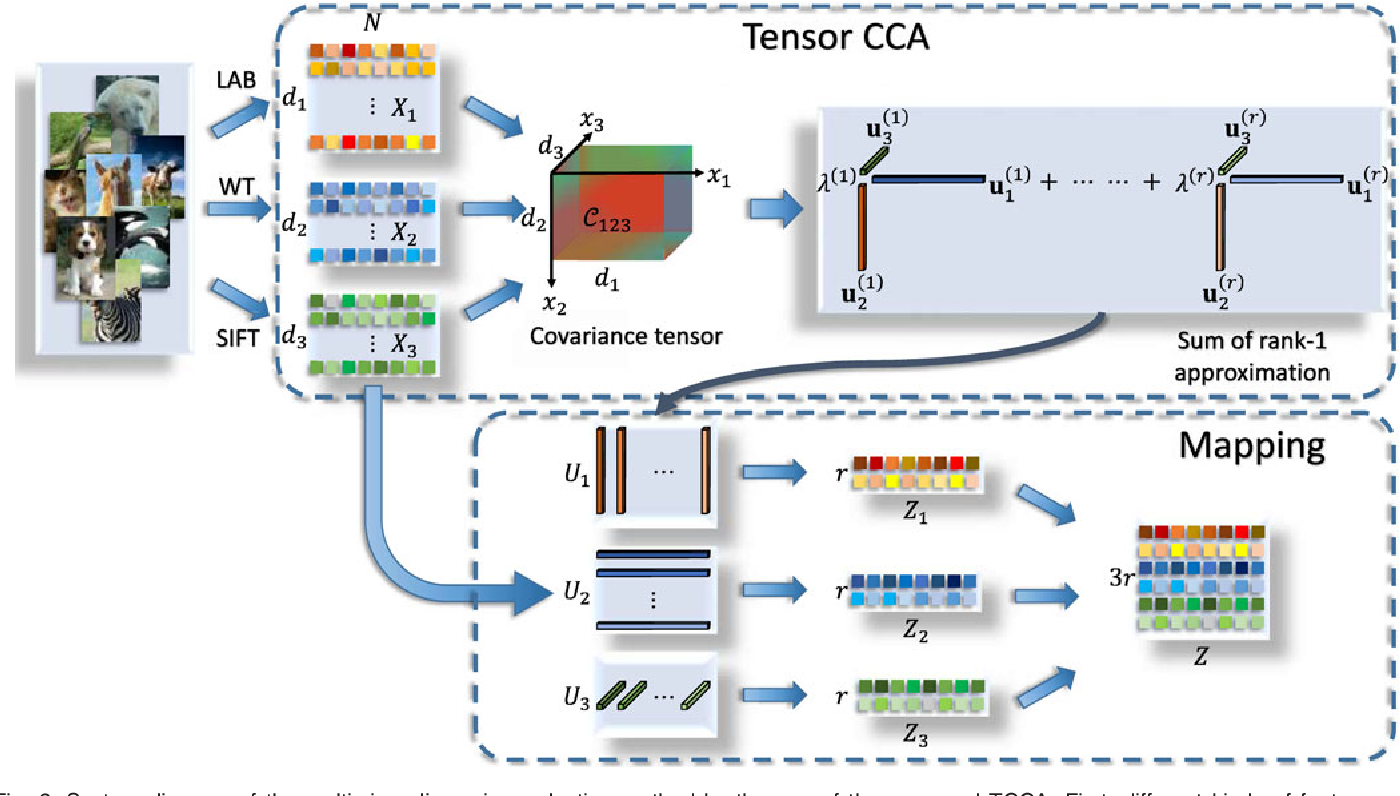
\includegraphics[width=\textwidth]{tensor-cca}
		\caption{Tensor CCA}
	\end{figure}
	
	Tensor Canonical Correlation Analysis (Tensor CCA) extends the traditional Canonical Correlation Analysis (CCA) to higher-dimensional tensor data, providing a method for analyzing relationships between two or more multi-dimensional arrays. In conventional CCA, the goal is to find linear transformations of two data matrices such that the transformed variables have maximum correlation. Tensor CCA generalizes this idea to tensors, enabling a more nuanced analysis of relationships in multi-way data, which is common in fields like neuroimaging, machine learning, and signal processing.
	
	\subsection{Problem notation}
	
	Given $m$ views $\{X_p\}_{p=1}^m$ of $N$ instances, where each $X_p = [x_{p1}, x_{p2}, \dots, x_{pN}] \in \mathbb{R}^{d_p \times N}$ is centered (i.e., has zero mean). The variance matrices are then defined as:
	\[
	C_{pp} = \frac{1}{N} \sum_{n=1}^N x_{pn} x_{pn}^T, \quad p = 1, \dots, m,
	\]
	and the covariance tensor among all views is calculated as:
	\[
	C_{12\ldots m} = \frac{1}{N} \sum_{n=1}^N x_{1n} \circ x_{2n} \circ \dots \circ x_{mn},
	\]
	where $C$ is a tensor of dimension $d_1 \times d_2 \times \dots \times d_m$. Following the objective of the traditional two-view CCA by Hardoon et al. (2004), the proposed tensor CCA seeks to maximize the correlation between the canonical variables $z_p = X_p^T h_p, p = 1, \dots, m$, where $\{h_p \in \mathbb{R}^{d_p \times 1}\}_{p=1}^m$ are usually called the canonical vectors. Therefore, the optimization problem is
	\[
	\underset{\{h_p\}}{\text{argmax }} \rho = \text{corr}(z_1, z_2, \dots, z_m)
	\]
	subject to $z_p^T z_p = 1, p = 1, \dots, m$.
	Here $\text{corr}(z_1, z_2, \dots, z_m) = (z_1 \odot z_2 \odot \dots \odot z_m)^T e$ is the canonical correlation, and $\odot$ denotes the element-wise product, where $e \in \mathbb{R}^N$ is an all-ones vector. We can prove that it is equivalent to $C_{12\ldots m} \times_1 h_1^T \times_2 h_2^T \dots \times_m h_m^T$, where $\times_p$ is the $p$-mode tensor-matrix product.
	
	\textbf{Theorem 1.} The high order canonical correlation is given by
	\[
	\rho = (z_1 \odot z_2 \odot \dots \odot z_m)^T e = C_{12\ldots m} \times_1 h_1^T \times_2 h_2^T \dots \times_m h_m^T.
	\]
	The proof is presented in the Appendix. By further considering that $X_p X_p^T = C_{pp}$ for $p = 1, \dots, m$, the problem becomes
	\[
	\underset{\{h_p\}}{\text{argmax }} \rho = C_{12\ldots m} \times_1 h_1^T \times_2 h_2^T \dots \times_m h_m^T
	\]
	subject to $h_p^T C_{pp} h_p = 1, p = 1, \dots, m$.
	To control model complexity, we add a regularization term to the constraints:
	\[
	h_p^T (C_{pp} + \epsilon I) h_p = 1, \quad p = 1, \dots, m,
	\]
	where $I$ is the identity matrix and $\epsilon$ is a nonnegative trade-off parameter. Let each $u_p = \tilde{C}_{pp}^{1/2} h_p$ and $\mathcal{M} = C_{12\ldots m} \times_1 \tilde{C}_{11}^{-1/2} \times_2 \tilde{C}_{22}^{-1/2} \dots \times_m \tilde{C}_{mm}^{-1/2}$, so that we can reformulate the problem as
	\[
	\underset{\{u_p\}}{\text{argmax }} \rho = \mathcal{M} \times_1 u_1^T \times_2 u_2^T \dots \times_m u_m^T
	\]
	subject to $u_p^T u_p = 1, \quad p = 1, \dots, m$.
	
	\subsection{Solutions}
	
	It has been presented in De Lathauwer et al. (2000b) that the problem is equivalent to finding the best rank-1 approximation of the tensor $\mathcal{M}$, i.e., if we define $\tilde{\mathcal{M}} = \rho u_1 \circ u_2 \circ \dots \circ u_m$, then the optimization problem becomes
	\[
	\underset{\{u_p\}}{\text{argmin }} \|\mathcal{M} - \tilde{\mathcal{M}}\|_F^2.
	\]
	The solution can be obtained using the alternating least square (ALS) algorithm. Other algorithms, such as the high-order power method (HOPM) and the tensor power method, can also be applied here for optimization.

	\begin{algorithm}
		\caption{Tensor Canonical Correlation Analysis (TCCA)}
		\label{alg:TCCA}
		\begin{algorithmic}
			\Procedure{TCCA}{$\{X_p\}_{p=1}^m$, $R$}
			\State Given $m$ views $\{X_p\}_{p=1}^m$ of $N$ instances, where each $X_p \in \mathbb{R}^{d_p \times N}$ and is centered (i.e., has zero mean).
			\State Compute the variance matrices for each view:
			\[
			C_{pp} = \frac{1}{N} \sum_{n=1}^N x_{pn} x_{pn}^T, \quad p = 1, \dots, m.
			\]
			\State Compute the covariance tensor among all views:
			\[
			C_{12\ldots m} = \frac{1}{N} \sum_{n=1}^N x_{1n} \circ x_{2n} \circ \dots \circ x_{mn}.
			\]
			\State Define the optimization problem:
			\[
			\underset{\{h_p\}}{\text{argmax }} \rho = \text{corr}(z_1, z_2, \ldots, z_m) = (z_1 \odot z_2 \odot \dots \odot z_m)^T e
			\]
			where $z_p = X_p^T h_p$, $p = 1, \dots, m$, and $\odot$ denotes the element-wise product.
			\State Solve for $\rho$ by iterating through the following steps:
			\begin{itemize}
				\item Update each canonical vector $h_p$ to maximize the correlation $\rho$ with constraints.
				\item Optionally, apply regularization to control model complexity:
				\[
				h_p^T (C_{pp} + \epsilon I) h_p = 1, \quad p = 1, \dots, m.
				\]
				\item Reformulate using transformed vectors $u_p$ such that $h_p = \tilde{C}_{pp}^{1/2} u_p$.
			\end{itemize}
			\State Return the canonical correlation $\rho$ and the projection vectors $\{u_p\}_{p=1}^m$.
			\EndProcedure
		\end{algorithmic}
	\end{algorithm}

	\section{Tensor CCA, variant 2}

	Tensor Canonical Correlation Analysis (Tensor CCA) is an advanced extension of Canonical Correlation Analysis (CCA) designed for higher-dimensional data. While standard CCA seeks linear relationships between two vector datasets, Tensor CCA generalizes this concept to tensors, enabling the modeling of relationships across multiple modes. This method is particularly useful for capturing correlations in spatiotemporal data, such as video or multi-view datasets.
	
	\subsection{Problem Statement}
	
	Given two tensors \( \mathcal{X} \in \mathbb{R}^{I_1 \times I_2 \times \dots \times I_N} \) and \( \mathcal{Y} \in \mathbb{R}^{J_1 \times J_2 \times \dots \times J_N} \), Tensor CCA seeks transformation matrices \( \mathbf{A}^{(n)} \) and \( \mathbf{B}^{(n)} \) for each mode \( n \) such that the transformed tensors maximize canonical correlations. Formally:
	\[
	\rho = \max_{\mathbf{A}^{(n)}, \mathbf{B}^{(n)}} \mathrm{corr} \left( \llbracket \mathcal{X}; \mathbf{A}^{(1)}, \mathbf{A}^{(2)}, \ldots, \mathbf{A}^{(N)} \rrbracket, \llbracket \mathcal{Y}; \mathbf{B}^{(1)}, \mathbf{B}^{(2)}, \ldots, \mathbf{B}^{(N)} \rrbracket \right),
	\]
	where:
	\begin{itemize}
		\item \( \mathbf{A}^{(n)} \in \mathbb{R}^{I_n \times d} \), \( \mathbf{B}^{(n)} \in \mathbb{R}^{J_n \times d} \), and \( d \) is the number of canonical components sought.
		\item \( \llbracket \cdot \rrbracket \) denotes the multilinear transformation applied along all modes.
	\end{itemize}
	Additionally, Tensor CCA returns multiple canonical correlations \( \rho_1, \ldots, \rho_d \), each corresponding to one of the canonical components.
	
	\begin{figure}
		\centering
		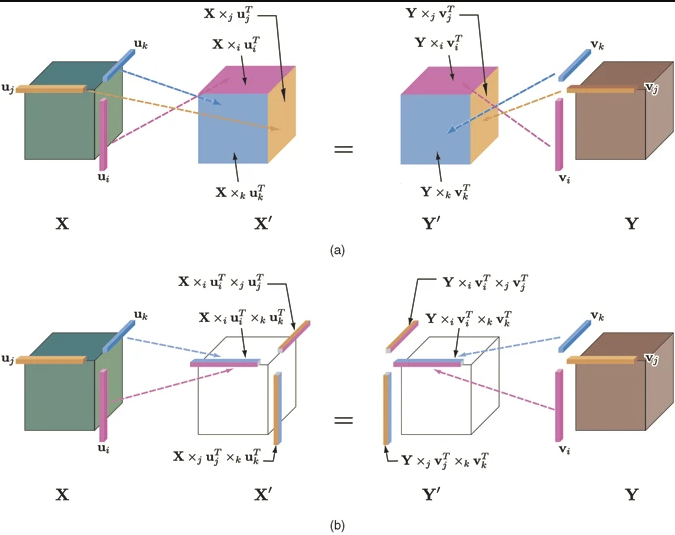
\includegraphics[width=\textwidth]{tensor-cca-2}
		\caption{Tensor CCA in 3 dimensions; (a) Joint-shared mode. (b) Single-shared mode}
	\end{figure}
	
	\subsection{Single-Shared-Mode TCCA Algorithm}
	
	The \textit{single-shared-mode} TCCA assumes the canonical components are aligned only along a single mode (e.g., the first mode) across the tensors. Here's the step-by-step algorithm:
	
	\begin{algorithm}
		\caption{Single-Shared-Mode Tensor CCA Algorithm}
		\label{alg:single_shared_mode_tcca}
		\begin{algorithmic}[1]
			\State \textbf{Input:} Tensors \( \mathcal{X}, \mathcal{Y} \), target dimension \( d \), max iterations \( T \), and tolerance \( \epsilon \).
			\State \textbf{Initialize:} Random orthogonal matrices \( \mathbf{A}^{(n)} \in \mathbb{R}^{I_n \times d} \), \( \mathbf{B}^{(n)} \in \mathbb{R}^{J_n \times d} \) for \( n = 1, \ldots, N \).
			\Repeat
			\For{each mode \( n = 1, \ldots, N \)}
			\State Unfold tensors \( \mathcal{X}_{(n)} \) and \( \mathcal{Y}_{(n)} \).
			\State Solve standard CCA for \( \mathcal{X}_{(n)} \) and \( \mathcal{Y}_{(n)} \).
			\State Compute canonical correlations \( \rho_1, \ldots, \rho_d \) and their corresponding canonical vectors.
			\State Update \( \mathbf{A}^{(n)} \) and \( \mathbf{B}^{(n)} \) using the canonical vectors.
			\EndFor
			\State Compute total canonical correlation \( \rho = \frac{1}{d} \sum_{i=1}^d \rho_i \).
			\Until{canonical correlations \( \rho \) converge or maximum iterations \( T \) are reached.}
			\State \textbf{Output:} Transformation matrices \( \mathbf{A}^{(n)} \), \( \mathbf{B}^{(n)} \), and canonical correlations \( \rho_1, \ldots, \rho_d \).
		\end{algorithmic}
	\end{algorithm}
	
	\subsection{Joined-Shared-Mode TCCA}
	
	In \textit{joined-shared-mode TCCA}, the canonical components are aligned along multiple or all modes simultaneously. This approach jointly optimizes the transformation matrices across all modes to find shared latent spaces.
	
	\begin{itemize}
		\item The optimization becomes more complex as the transformations for all modes are coupled.
		\item The canonical correlations \( \rho_1, \ldots, \rho_d \) are computed by jointly maximizing the correlation across the unfolded tensors of all modes.
		\item Mathematically, the correlation matrix is constructed across all modes, and \( \rho_1, \ldots, \rho_d \) are derived from the leading eigenvalues of this matrix.
	\end{itemize}

	\section{Conclusion}
	This essay presented CP and Tucker decompositions and introduced Tensor CCA for multi-view correlation analysis. These tensor models enable advanced dimensionality reduction and efficient data representation in multidimensional settings, supporting numerous applications in data-intensive fields.
	
	\nocite{*}
	\printbibliography
	
\end{document}
